% ============================================================
%  Chapter 1 — Introduction
% ============================================================
\chapter{Introduction}
\label{ch:intro}

When we look at a white wall, we see the same white whether part of it is in shadow or
in direct light.
Our visual system separates the lightness and colour of a surface from the light falling on
it, and this ability, called \emph{lightness and colour constancy}, is so automatic that we
rarely think about it.
For computers, it is a hard problem.
A camera simply records the product of surface reflectance and illumination, and the two
are mixed together in every pixel.
Separating them is the goal of \emph{Intrinsic Image Decomposition} (IID).

IID has a long history in computer vision and colour science, dating back to the
Retinex theory of \mycitetext{land71retinex}.
The core idea is that a photograph $\mathbf{I}$ can be modelled as the product of
two layers: an \emph{albedo} $\mathbf{A}$ and a \emph{shading} $S$.
\begin{equation}
  \mathbf{I}(p) = \mathbf{A}(p) \cdot S(p), \qquad \forall\, p \in \Omega
  \label{eq:iid_model}
\end{equation}
Here $p$ denotes a pixel, $\Omega$ is the set of all pixels, the albedo encodes
the true material colour at each pixel, and the shading encodes how bright the
surface is due to lighting and geometry.
Throughout this report, ``material colour'' means this diffuse albedo in linear RGB, not the
spectral reflectance of the surface.
If we can recover $\mathbf{A}$ reliably, we obtain a lighting-independent
description of the scene. This separation has practical consequences. An
interior-design tool can recolour a wall without painting over its shadows; an
augmented-reality system can place a virtual chair under the room's existing
light; a photograph can be re-lit without changing the apparent material; and a
catalogue or inspection system can compare product colours captured under
different lamps. All four applications fail when the lighting, its brightness
pattern or its colour, remains baked into the estimated material.

\begin{figure}[t!]
  \centering
  \begin{minipage}[t]{0.235\textwidth}\centering
    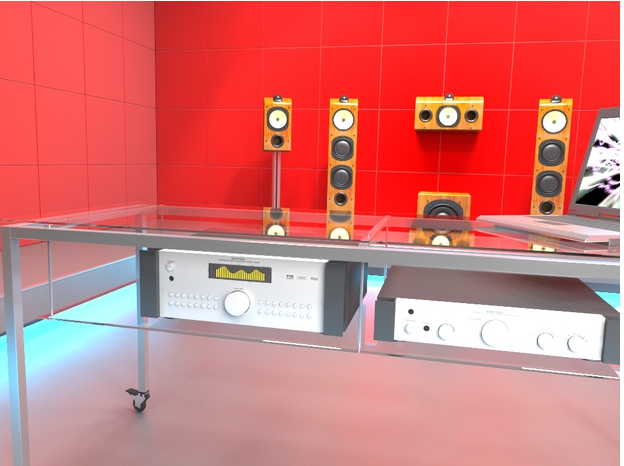
\includegraphics[width=\linewidth]{images/intro/input.png}\\[-1mm]
    \small Photograph $\mathbf{I}$
  \end{minipage}\hfill
  \begin{minipage}[t]{0.235\textwidth}\centering
    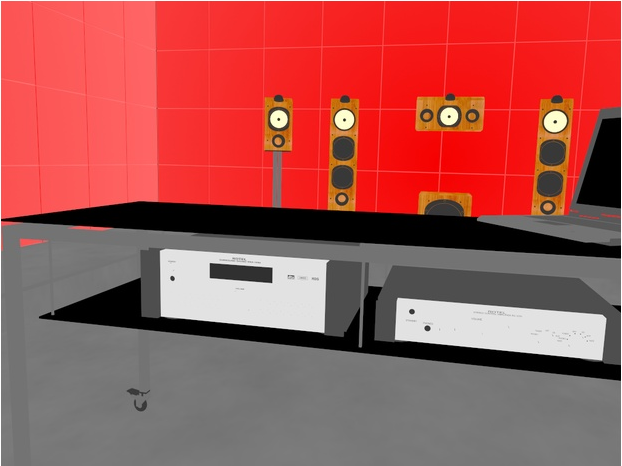
\includegraphics[width=\linewidth]{images/intro/albedo.png}\\[-1mm]
    \small Albedo $\mathbf{A}$
  \end{minipage}\hfill
  \begin{minipage}[t]{0.235\textwidth}\centering
    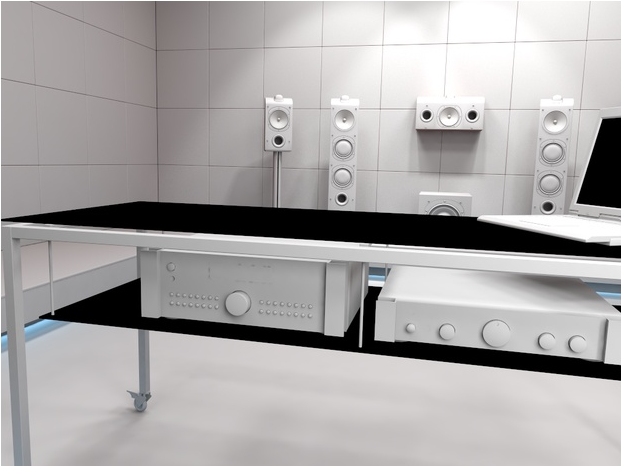
\includegraphics[width=\linewidth]{images/intro/shading.png}\\[-1mm]
    \small Diffuse shading $\mathbf{S}_d$
  \end{minipage}\hfill
  \begin{minipage}[t]{0.235\textwidth}\centering
    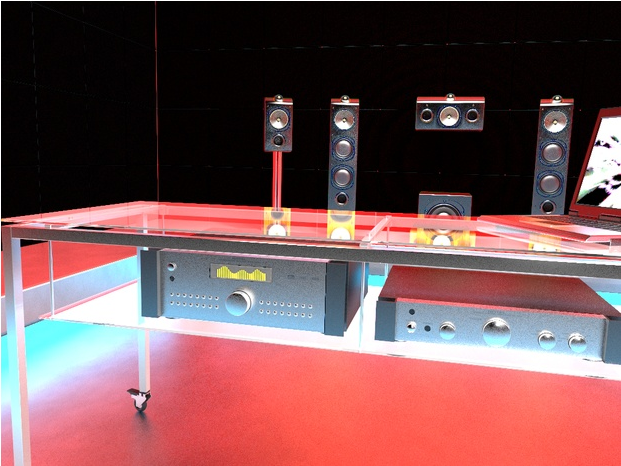
\includegraphics[width=\linewidth]{images/intro/residual.png}\\[-1mm]
    \small Residual $\mathbf{R}$
  \end{minipage}
  \caption[A photograph and its ground-truth decomposition.]{%
    One rendered image from Hypersim \mycite{roberts21hypersim} and its ground-truth layers.
    The renderer separates the image into the albedo, the diffuse shading and a non-diffuse
    residual, so that $\mathbf{I} = \mathbf{A} \odot \mathbf{S}_d + \mathbf{R}$.
    The residual holds what a diffuse material times shading cannot explain, here the
    reflections in the glass table, the lit display and the specular highlights on the
    loudspeakers. It is shown at three times its value.
  }
  \label{fig:intro_layers}
\end{figure}

This thesis started from one such application. It was carried out at 3DUniversum, where
photographs of interiors, for example for real-estate listings, often need to be enhanced:
the dark corners should be brighter and the lighting more even, while walls, floors and
furniture keep their real appearance. Editing the pixels directly cannot do this well. A
pixel does not tell whether it is dark because it lies in a shadow or because the material
itself is dark, so brightening the image lifts a shadowed wall and a dark lamp by the same
amount, and the lamp turns grey (\figref{fig:intro_enhance}, middle). IID offers a cleaner
route: brighten only the shading layer and keep the albedo as it is
(\figref{fig:intro_enhance}, right). This route works only if the albedo is free of
lighting. A shadow or a bright patch that stays in the albedo cannot be reached by a
shading edit, so it stays in the enhanced photograph too. An albedo that does not change
with the light is therefore the goal of this thesis, and \chapref{ch:practice} returns to
this example.

\begin{figure}[t!]
  \centering
  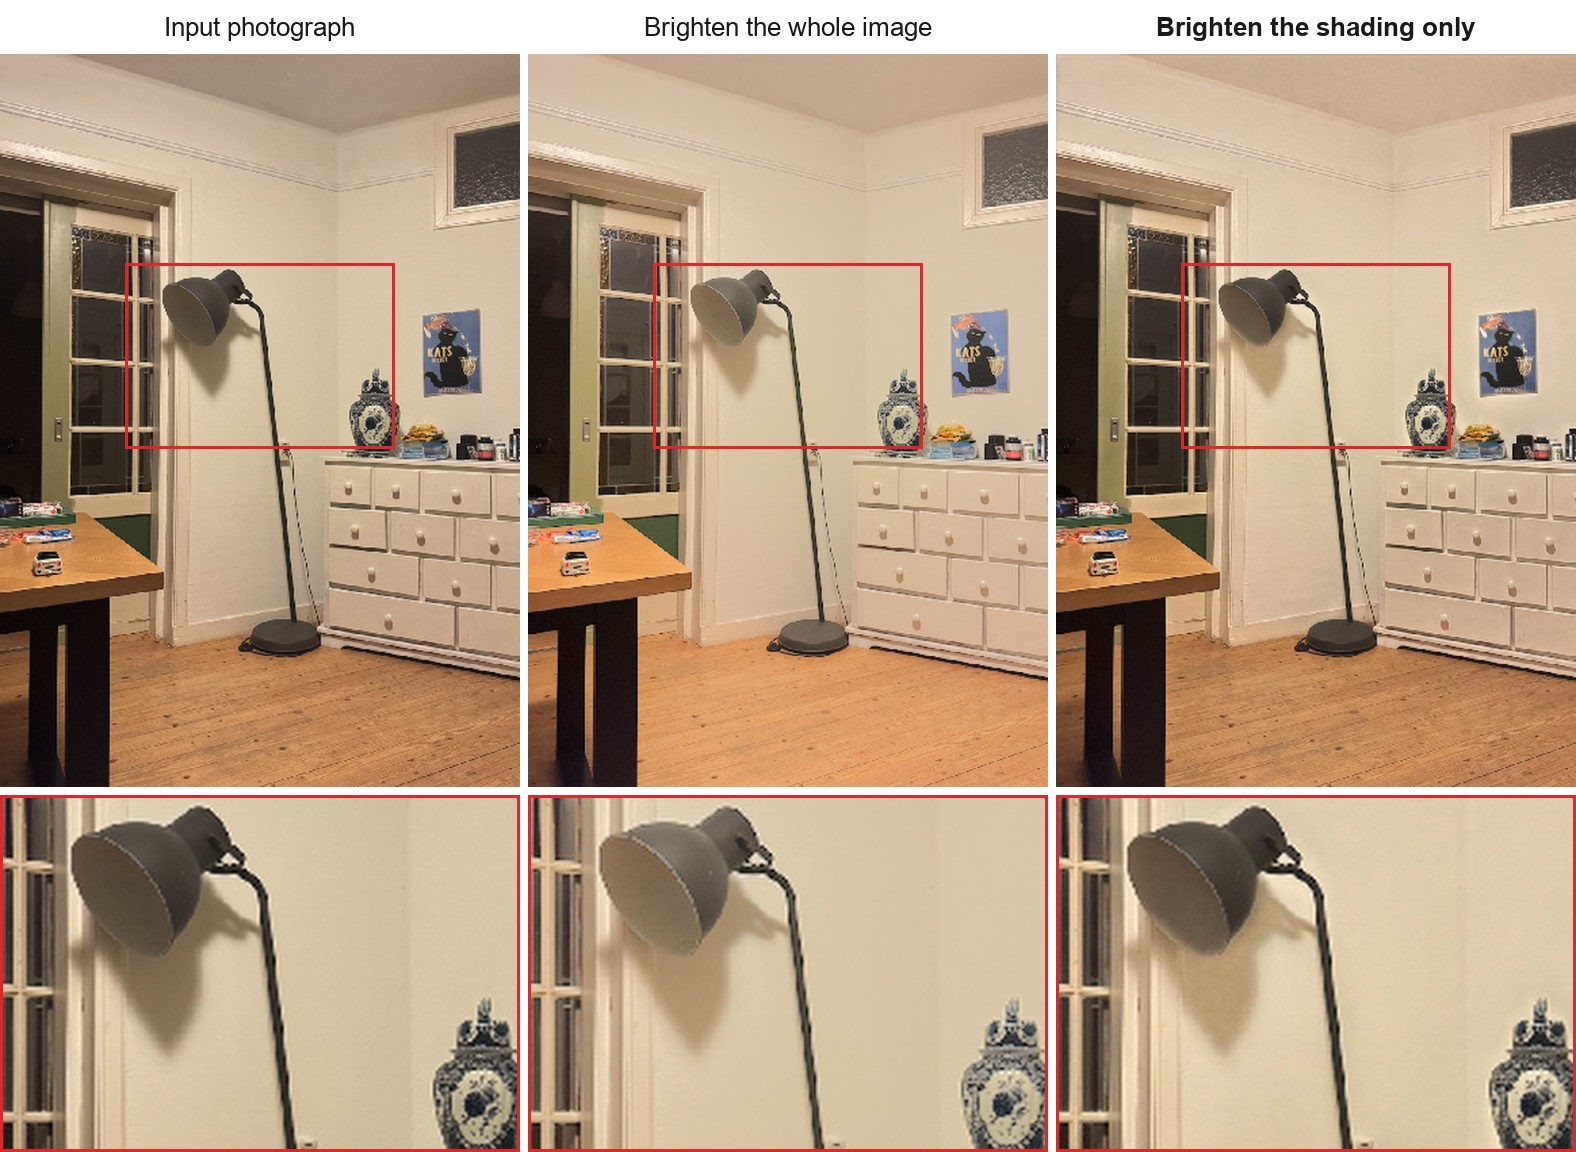
\includegraphics[width=\textwidth]{images/ch6/enhance.jpg}
  \caption[Why a clean albedo matters for photo enhancement.]{%
    Why a clean albedo matters for photo enhancement. \emph{Left:} an indoor photograph.
    \emph{Middle:} a brightness gain that is large on dark pixels, applied to the whole
    image. It also lifts dark materials, so the dark lamp and the window turn grey.
    \emph{Right:} the same kind of gain computed from our predicted shading and applied to
    the shading only, with the albedo and residual unchanged. The shadow of the lamp on the
    wall becomes lighter while the lamp keeps its colour. Bottom row: $2\times$ crops of the
    red box. The edit is defined in \secref{sec:factor_edit}.
  }
  \label{fig:intro_enhance}
\end{figure}

\section{The Problem: Lighting Leaks into the Albedo}
\label{sec:intro_problem}

\eqnref{eq:iid_model} has twice as many unknowns as observations, so every IID method
relies on priors to choose one factorisation. When those priors fail, part of the
lighting is assigned to the albedo. Two forms of this leakage matter here.

The first is \emph{luminance} leakage. A shadow, a soft gradient from a nearby lamp or a
bright patch where light falls directly can be read as a darker or lighter material.
The same wall then receives a different albedo depending on where the light comes from,
even if the light is white.

The second is \emph{colour} leakage. Most IID methods, classical and modern, assume a grey
illuminant, so that the shading $S$ in \eqnref{eq:iid_model} is one value per pixel and all
colour in the image is attributed to the albedo. Real indoor light is rarely grey:
incandescent bulbs are warm, LEDs can be cool, and light bounced off a coloured wall takes
on its colour. With a scalar shading the illuminant hue has nowhere to go but the albedo,
and even with a three-channel shading a single image does not say how much of a hue belongs
to the surface and how much to the light.

\figref{fig:intro_constancy} shows the setting used in this work: one real scene
photographed under several flash directions, and the albedo our model predicts from each
photograph on its own. Where the map turns red, the predicted material changes with the
light, which is exactly the leakage described above.

\begin{figure}[t!]
  \centering
  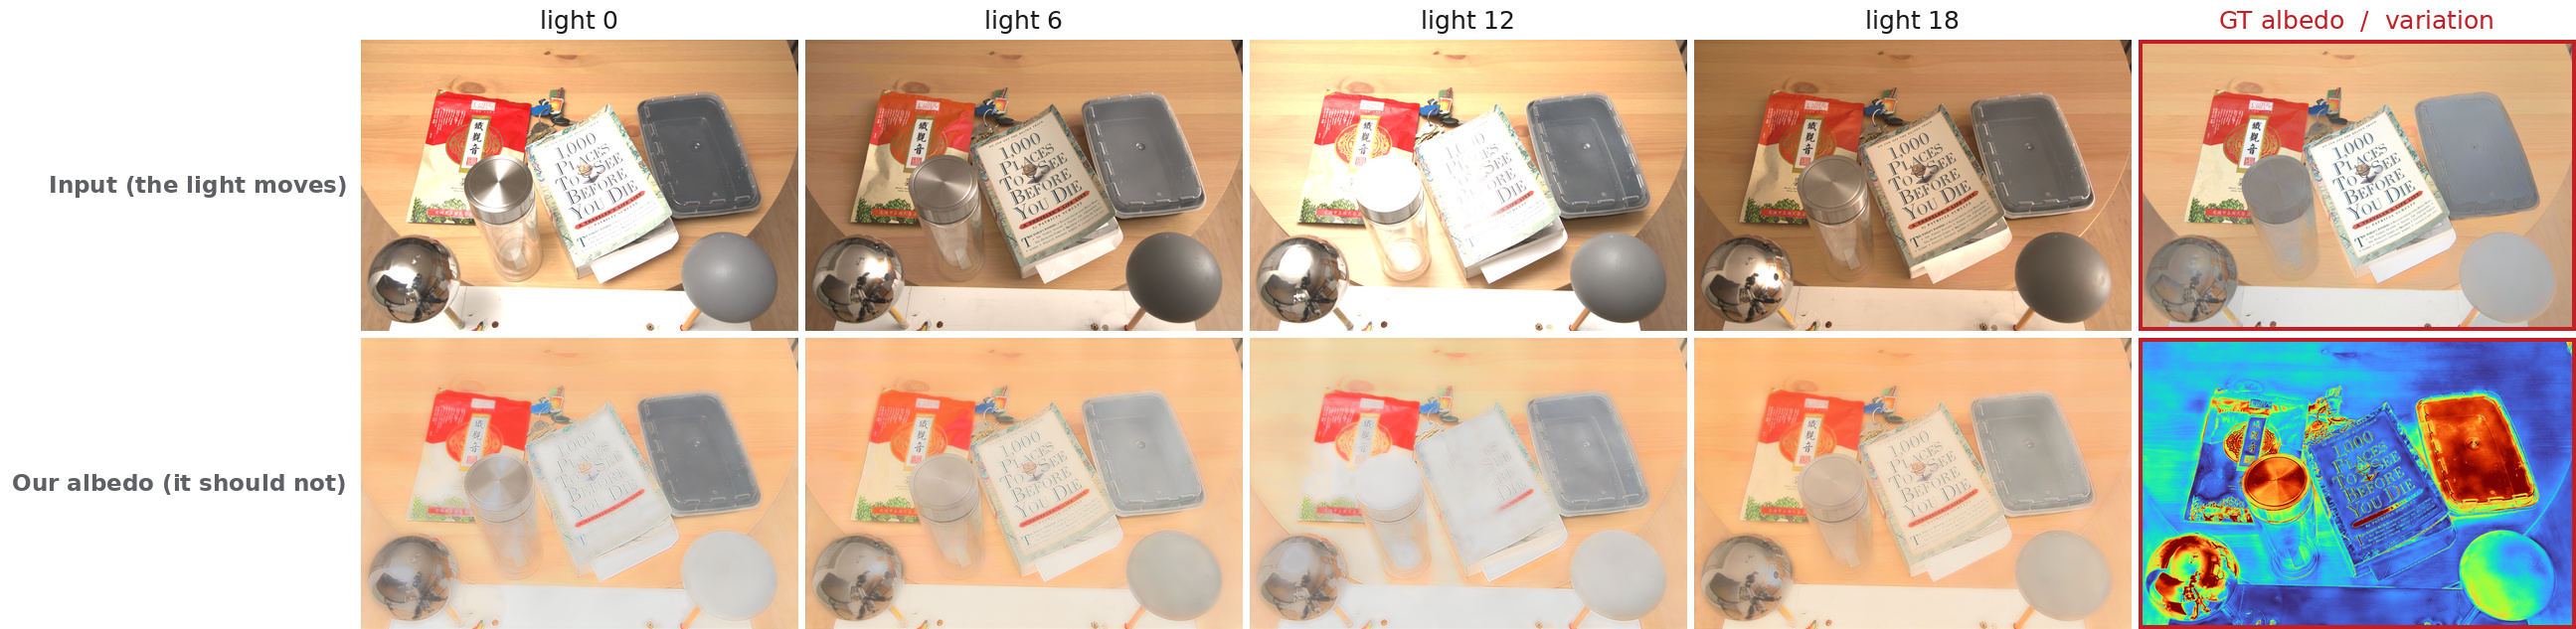
\includegraphics[width=\textwidth]{images/hires/mid_ours.jpg}
  \caption[MID albedo predictions under four flash directions.]{%
    Albedo predictions on one MID scene under four flash directions.
    The upper row shows the four inputs and the dataset pseudo-ground-truth albedo;
    the lower row shows the four predictions and a per-pixel coefficient-of-variation
    map of predicted luminance (red marks regions that change with the light).
    The map stays cool over the table and most matte surfaces, and turns red on the
    plastic tray, the glass jar and the mirror sphere.
  }
  \label{fig:intro_constancy}
\end{figure}

\paragraph{Goal}
The goal of this thesis is a model that predicts, from a single photograph, an albedo whose
luminance stays the same when only the light changes, without losing the colour of the
material. We call the first property \emph{stability} and the second \emph{accuracy}.
We also measure how far the same approach carries to the colour of the albedo.


\section{Why the Problem Is Hard}
\label{sec:intro_challenges}

Four difficulties shape the design of this work.

\begin{enumerate}
  \item \textbf{One image is ambiguous.} A dark surface in bright light and a bright surface
  in shadow can produce the same pixel. A model must learn priors, and priors learned on
  synthetic renderings do not always transfer to real rooms.

  \item \textbf{Real photographs have no albedo ground truth.} Dense albedo can be measured
  only in rendered scenes. For real photographs we have at most a pseudo-ground truth or
  sparse human judgements, so we cannot simply show the model the right answer on real data.

  \item \textbf{Stability alone has a trivial solution.} A model that outputs the same flat
  grey albedo for every image is perfectly stable and completely wrong
  (\figref{fig:intro_trivial}). Any loss or score that rewards stability must therefore be
  paired with something that rewards accuracy.

  \item \textbf{Real multi-illumination data varies the light in the wrong way for colour.}
  The only real dataset with many lights per scene and a dense pseudo-ground truth is MID
  \mycite{midintrinsics}. Its flash is white, so between two frames the light changes in
  direction and intensity, but its colour changes only through light bounced off coloured
  surfaces: the median chromaticity gap between two frames of a scene is $0.030$. MID can
  teach luminance well and colour only weakly.
\end{enumerate}

A practical constraint is added to these: all training runs on a single 24\,GB GPU.

\begin{figure}[t!]
  \centering
  \tikzset{
    pics/alb/.style n args={3}{code={
      \path[#1] (0,0) rectangle (0.55,1.1);
      \path[#2] (0.55,0) rectangle (1.1,1.1);
      \path[#3] (1.1,0) rectangle (1.65,1.1);
      \draw[black!55] (0,0) rectangle (1.65,1.1);
    }}
  }
  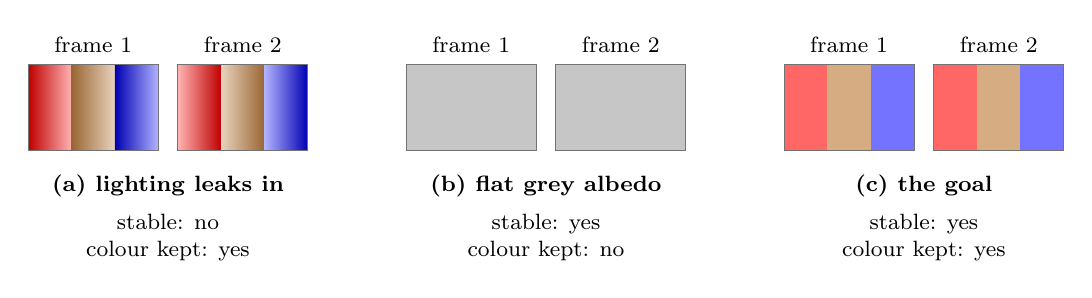
\begin{tikzpicture}[lab/.style={font=\footnotesize, align=center}]
    % (a) lighting leaks into the albedo: the brightness gradient follows the light
    \pic at (0,0)    {alb={{left color=red!75!black, right color=red!30}}{{left color=brown!80!black, right color=brown!35}}{{left color=blue!70!black, right color=blue!30}}};
    \pic at (1.9,0)  {alb={{left color=red!30, right color=red!75!black}}{{left color=brown!35, right color=brown!80!black}}{{left color=blue!30, right color=blue!70!black}}};
    % (b) flat grey albedo: identical, but the materials are gone
    \pic at (4.8,0)  {alb={fill=gray!45}{fill=gray!45}{fill=gray!45}};
    \pic at (6.7,0)  {alb={fill=gray!45}{fill=gray!45}{fill=gray!45}};
    % (c) goal: identical and with the true material colours
    \pic at (9.6,0)  {alb={fill=red!60}{fill=brown!65}{fill=blue!55}};
    \pic at (11.5,0) {alb={fill=red!60}{fill=brown!65}{fill=blue!55}};
    \foreach \x in {0,4.8,9.6} {
      \node[lab] at (\x+0.825,1.35) {frame 1};
      \node[lab] at (\x+2.725,1.35) {frame 2};
    }
    \node[lab] at (1.775,-0.45)  {\textbf{(a) lighting leaks in}};
    \node[lab] at (6.575,-0.45)  {\textbf{(b) flat grey albedo}};
    \node[lab] at (11.375,-0.45) {\textbf{(c) the goal}};
    \node[lab] at (1.775,-1.1)  {stable: no\\colour kept: yes};
    \node[lab] at (6.575,-1.1)  {stable: yes\\colour kept: no};
    \node[lab] at (11.375,-1.1) {stable: yes\\colour kept: yes};
  \end{tikzpicture}
  \caption[Why stability must be read beside accuracy.]{%
    Three ways a model can predict the albedo of the same three materials from two
    photographs taken under different light (schematic). (a) The brightness pattern of the
    light stays in the albedo, so the prediction changes between frames. (b) A flat grey
    albedo is identical in both frames, so it is perfectly stable, but every material has
    lost its colour. (c) The goal is stable \emph{and} accurate. A stability loss alone cannot
    tell (b) from (c); this is why CIAI has a second loss and why every stability score in
    this thesis is reported beside an accuracy score.
  }
  \label{fig:intro_trivial}
\end{figure}


\section[Our Idea: Cross-Illumination Albedo Invariance]{Our Idea: Cross-Illumination\newline Albedo Invariance}
\label{sec:intro_idea}

The four difficulties point to one observation. If we photograph the same scene twice under
different light, the surfaces are identical in the two images, so whatever differs between
them is lighting. A second photograph therefore carries a training signal that needs no
albedo ground truth.

We turn this observation into a training strategy and call it
\emph{Cross-Illumination Albedo Invariance} (CIAI).
Two photographs of one scene under different illumination are passed through the same
network. An invariance loss requires the two predicted albedos to agree, and an explanation
loss requires the ratio of the two predicted shadings to match the luminance ratio of the
two images, so that the model cannot satisfy the first loss with a flat albedo.
The pairing is needed only during training; at inference the model takes one image.

\begin{figure}[t!]
  \centering
  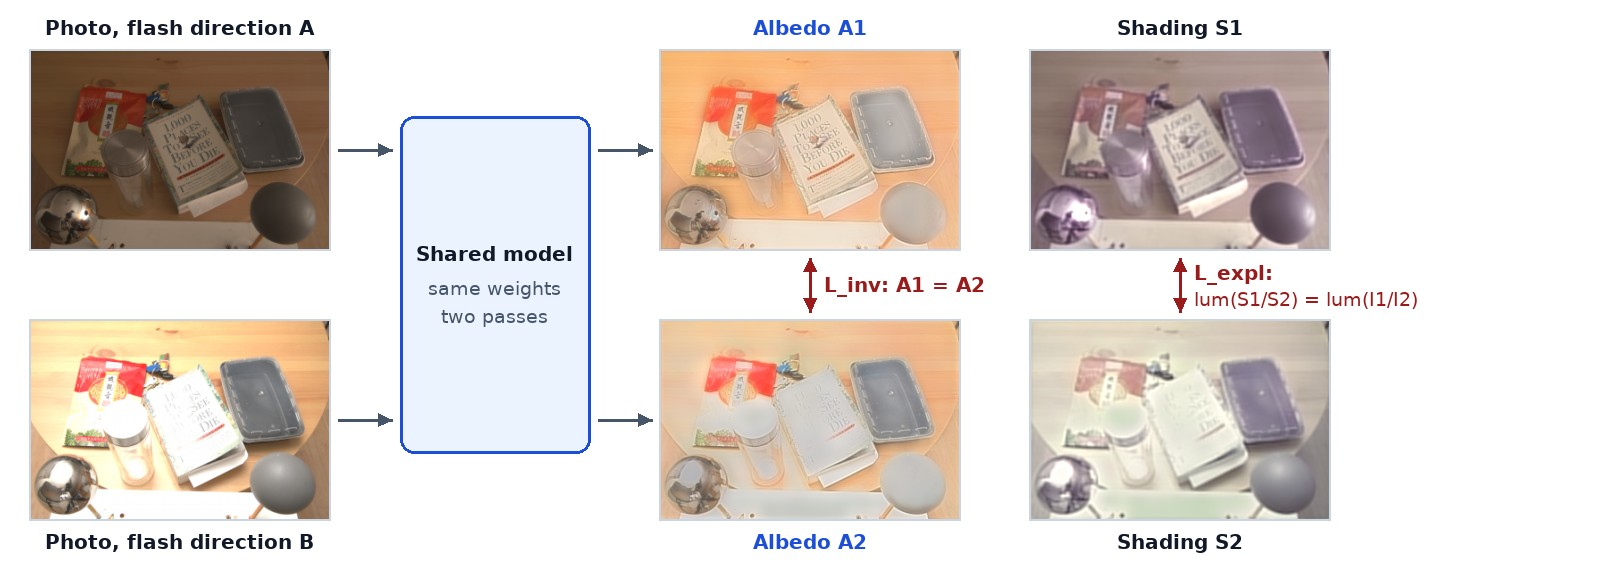
\includegraphics[width=0.92\textwidth]{images/intro/ciai_mechanism.jpg}
  \caption[The CIAI idea in one picture.]{%
    The idea of CIAI. Two photographs of one scene, taken with the flash in two
    directions, pass through the same model. The two predicted albedos are tied by the
    invariance loss $\mathcal{L}_{\text{inv}}$, and the two predicted shadings by the
    explanation loss $\mathcal{L}_{\text{expl}}$. \secref{sec:ciai} defines both losses.
  }
  \label{fig:intro_ciai}
\end{figure}

The idea is borrowed from two places. Siamese and contrastive representation learning train
a network so that two views of the same object map to the same representation
\mycite{chen21simsiam}; multi-view 3D reconstruction asks one surface, observed several
times, to receive one set of properties. CIAI keeps only positive pairs, with no negatives,
and replaces the learned embedding by a dense, physically defined target: the albedo map.
Training IID on images of one scene under varying light is not new in itself; time-lapse and
illumination-varying sequences have been used for self-supervised decomposition
\mycite{li18bigtime,lettry18unsupervised,ma18single,kinoshita21consistency}. What we study is
the effect of this constraint as a fine-tuning stage on top of supervised synthetic training
in a modern feed-forward model, using real raw photographs, and what such pairs can and
cannot teach.


\section{How We Solve It}
\label{sec:intro_solution}

We implement CIAI inside a model built on a frozen \emph{DINOv2-Large} vision encoder
\mycite{oquab24dinov2} and a Dense Prediction Transformer (DPT) decoder
\mycite{ranftl21dpt} with a three-channel shading output.
The model is first trained with supervised losses on the synthetic datasets Hypersim
\mycite{roberts21hypersim} and InteriorVerse \mycite{zhu22interiorverse}; CIAI is then added
in a second stage on real MID pairs, with the pseudo-ground-truth albedo that MIDIntrinsics
derives for every MID scene \mycite{careaga23ordinal}.
\tabref{tab:intro_plan} shows how each difficulty of \secref{sec:intro_challenges} is
answered.

\begin{table}[t!]
  \caption[How each difficulty is addressed.]{%
    The difficulties of \secref{sec:intro_challenges} and the part of our approach that
    answers each one.}
  \label{tab:intro_plan}
  \centering
  \small
  \begin{tabular}{@{}>{\raggedright\arraybackslash}p{0.27\textwidth}>{\raggedright\arraybackslash}p{0.52\textwidth}>{\raggedright\arraybackslash}p{0.13\textwidth}@{}}
    \toprule
    Difficulty & Our answer & Where \\
    \midrule
    One image is ambiguous
      & Start from a strong pretrained encoder and learn the priors with supervised losses
        on synthetic data before any pair is used.
      & \secref{sec:architecture}, \secref{sec:schedule} \\
    No albedo ground truth for real photographs
      & Use the pair itself as supervision: the two predicted albedos must agree
        ($\mathcal{L}_{\text{inv}}$).
      & \secref{sec:ciai} \\
    Stability has a trivial solution
      & The shading must explain the change in light ($\mathcal{L}_{\text{expl}}$); one frame
        of each pair stays supervised; every stability score is reported beside an accuracy
        score.
      & \secref{sec:ciai}, \secref{sec:metrics} \\
    MID varies colour very little
      & Keep the second frame raw so that the small colour change survives; claim only
        luminance stability; measure the colour range and test whether hue drift follows it.
      & \secref{sec:raw_pairs}, \secref{sec:colour_axis} \\
    One 24\,GB GPU
      & Freeze the encoder and train $18.5$M parameters; pairs are used only in training,
        so inference is one image and one forward pass.
      & \secref{sec:schedule} \\
    \bottomrule
  \end{tabular}
\end{table}

These choices follow from the data. MID is used because it is the only real dataset with
many illuminations per scene and a dense albedo reference. The explanation loss is defined
on luminance because MID's pairs differ mainly in brightness, so a colour term would mostly fit
noise. The encoder is frozen because it gives strong features at
a cost that fits one GPU, and because it lets the effect of CIAI be measured on a fixed
backbone.


\section{Contributions}

The contributions of this work are:

\begin{enumerate}

  \item \textbf{A paired training strategy on real photographs} (\secref{sec:ciai}).
  An albedo-invariance loss and a luminance explanation loss on raw MID pairs with
  pseudo-ground-truth albedo, added as a second training stage. The pairs are needed only in
  training, so inference stays one image and one forward pass, and the model trains $18.5$M
  parameters on top of a frozen encoder.

  \item \textbf{Matched evidence for what it changes} (\secref{sec:ablation}).
  A $2 \times 2$ ablation from one shared checkpoint isolates the effect of CIAI. In our final
  model it cuts the variation of recovered material luminance across illuminations by $39\%$,
  and it lowers the dense albedo error (LMSE) on raw ARAP renderings, a benchmark it never
  trained on, by $7\%$. The gain in hue stability is small, and we measure why
  (\secref{sec:colour_axis}).

  \item \textbf{An evaluation that reports stability next to accuracy} (\secref{sec:metrics}).
  Material-level stability on MID is always read beside accuracy against measured albedo
  (MAW) and against the MID pseudo-ground truth, so that a flat albedo cannot score well
  (\figref{fig:intro_trivial}).

\end{enumerate}
\chapref{ch:conclusion} sets out the next stage of the work, a model that separates shading
luminance from shading chroma so that colour can be learned as well.

The project code, training configurations, and evaluation scripts are publicly available at
\url{https://github.com/tmkhang1999/CIAI}.

The rest of this report is organised as follows.
\chapref{ch:related} reviews related work on IID, paired-illumination training,
multi-illuminant scenes, and the evaluation benchmarks.
\chapref{ch:method} describes the model architecture and the CIAI training strategy.
\chapref{ch:implementation} covers the loss terms, training data, and optimisation
schedule in detail.
\chapref{ch:experiments} presents the benchmark results, the ablation, and the colour
limitation.
\chapref{ch:practice} demonstrates qualitative factor edits built directly on the
decomposition.
\chapref{ch:conclusion} summarises the findings, discusses limitations, and
sets out the next stage of the work.
